\chapter{Pre-Lab Exercises}

\section{Exercise \#1}

\begin{table}[h]
    \centering
    \begin{tabular}{|c|c|c|c|c|c|}
        \hline
        Color   & 1st Band & 2nd Band & 3rd Band & Multiplier (\(\Omega\)) & Tolerance (\%) \\ \hline
        Black   & 0        & 0        & 0        & 1                     & -              \\ \hline
        Brown   & 1        & 1        & 1        & 10                    & \(\pm\)1       \\ \hline
        Red     & 2        & 2        & 2        & 100                   & \(\pm\)2       \\ \hline
        Orange  & 3        & 3        & 3        & 1,000                 & -              \\ \hline
        Yellow  & 4        & 4        & 4        & 10,000                & -              \\ \hline
        Green   & 5        & 5        & 5        & 100,000               & \(\pm\)0.5     \\ \hline
        Blue    & 6        & 6        & 6        & 1,000,000             & \(\pm\)0.25    \\ \hline
        Violet  & 7        & 7        & 7        & 10,000,000            & \(\pm\)0.1     \\ \hline
        Gray    & 8        & 8        & 8        & 100,000,000           & \(\pm\)0.05    \\ \hline
        White   & 9        & 9        & 9        & 1,000,000,000         & -              \\ \hline
        Gold    & -        & -        & -        & 0.1                   & \(\pm\)5       \\ \hline
        Silver  & -        & -        & -        & 0.01                  & \(\pm\)10      \\ \hline
    \end{tabular}
    \caption{Resistor Color Code Table \cite{resistor-calculator}}
\end{table}

In order to calculate the resistance value of a resistor using the color code, we can use the following formula:

\[
    \text{Resistance} = (1^{st}~\text{Band} \times 10 + 2^{nd}~\text{Band}) \times \text{Multiplier}
\]

For example, let's calculate the resistance value of a resistor with the color code of \textbf{Red, Red, Orange}:

\[
    \text{Resistance} = (2 \times 10 + 2) \times 1,000 = 22k\Omega
\]

\newpage
\thispagestyle{plain}

For example, in order to find the color code of the resistor with the resistance value of 4.7k\(\Omega\), we can use the following formula:

\begin{align*}
    1^{st}~\text{Band} &= \text{First significant digit} = 4 \\
    2^{nd}~\text{Band} &= \text{Second significant digit} = 7 \\
    3^{rd}~\text{Band} &= 10^{\text{Number of zeros in the resistance value}} = 10^3 = 1,000 \\
    \text{Color Code} &= \text{Yellow-Violet-Red}
\end{align*}


\bigbreak{}
\bigbreak{}

Let's find the color code of these $3$ resistors:
\begin{table}[h]
    \centering
    \begin{tabular}{|c|c|}
    \hline
    Resistor & Color Code \\
    \hline
    \(R_1 = 470\Omega\) & Yellow-Violet-Brown \\
    \(R_2 = 1k\Omega\) & Brown-Black-Red \\
    \(R_3 = 4.3k\Omega\) & Yellow-Orange-Red \\
    \hline
    \end{tabular}
    \caption{Color Codes for Given Resistors}
\end{table}

\newpage
\thispagestyle{plain}

\section{Exercise \#2}

\begin{figure}[h]
    \centering
    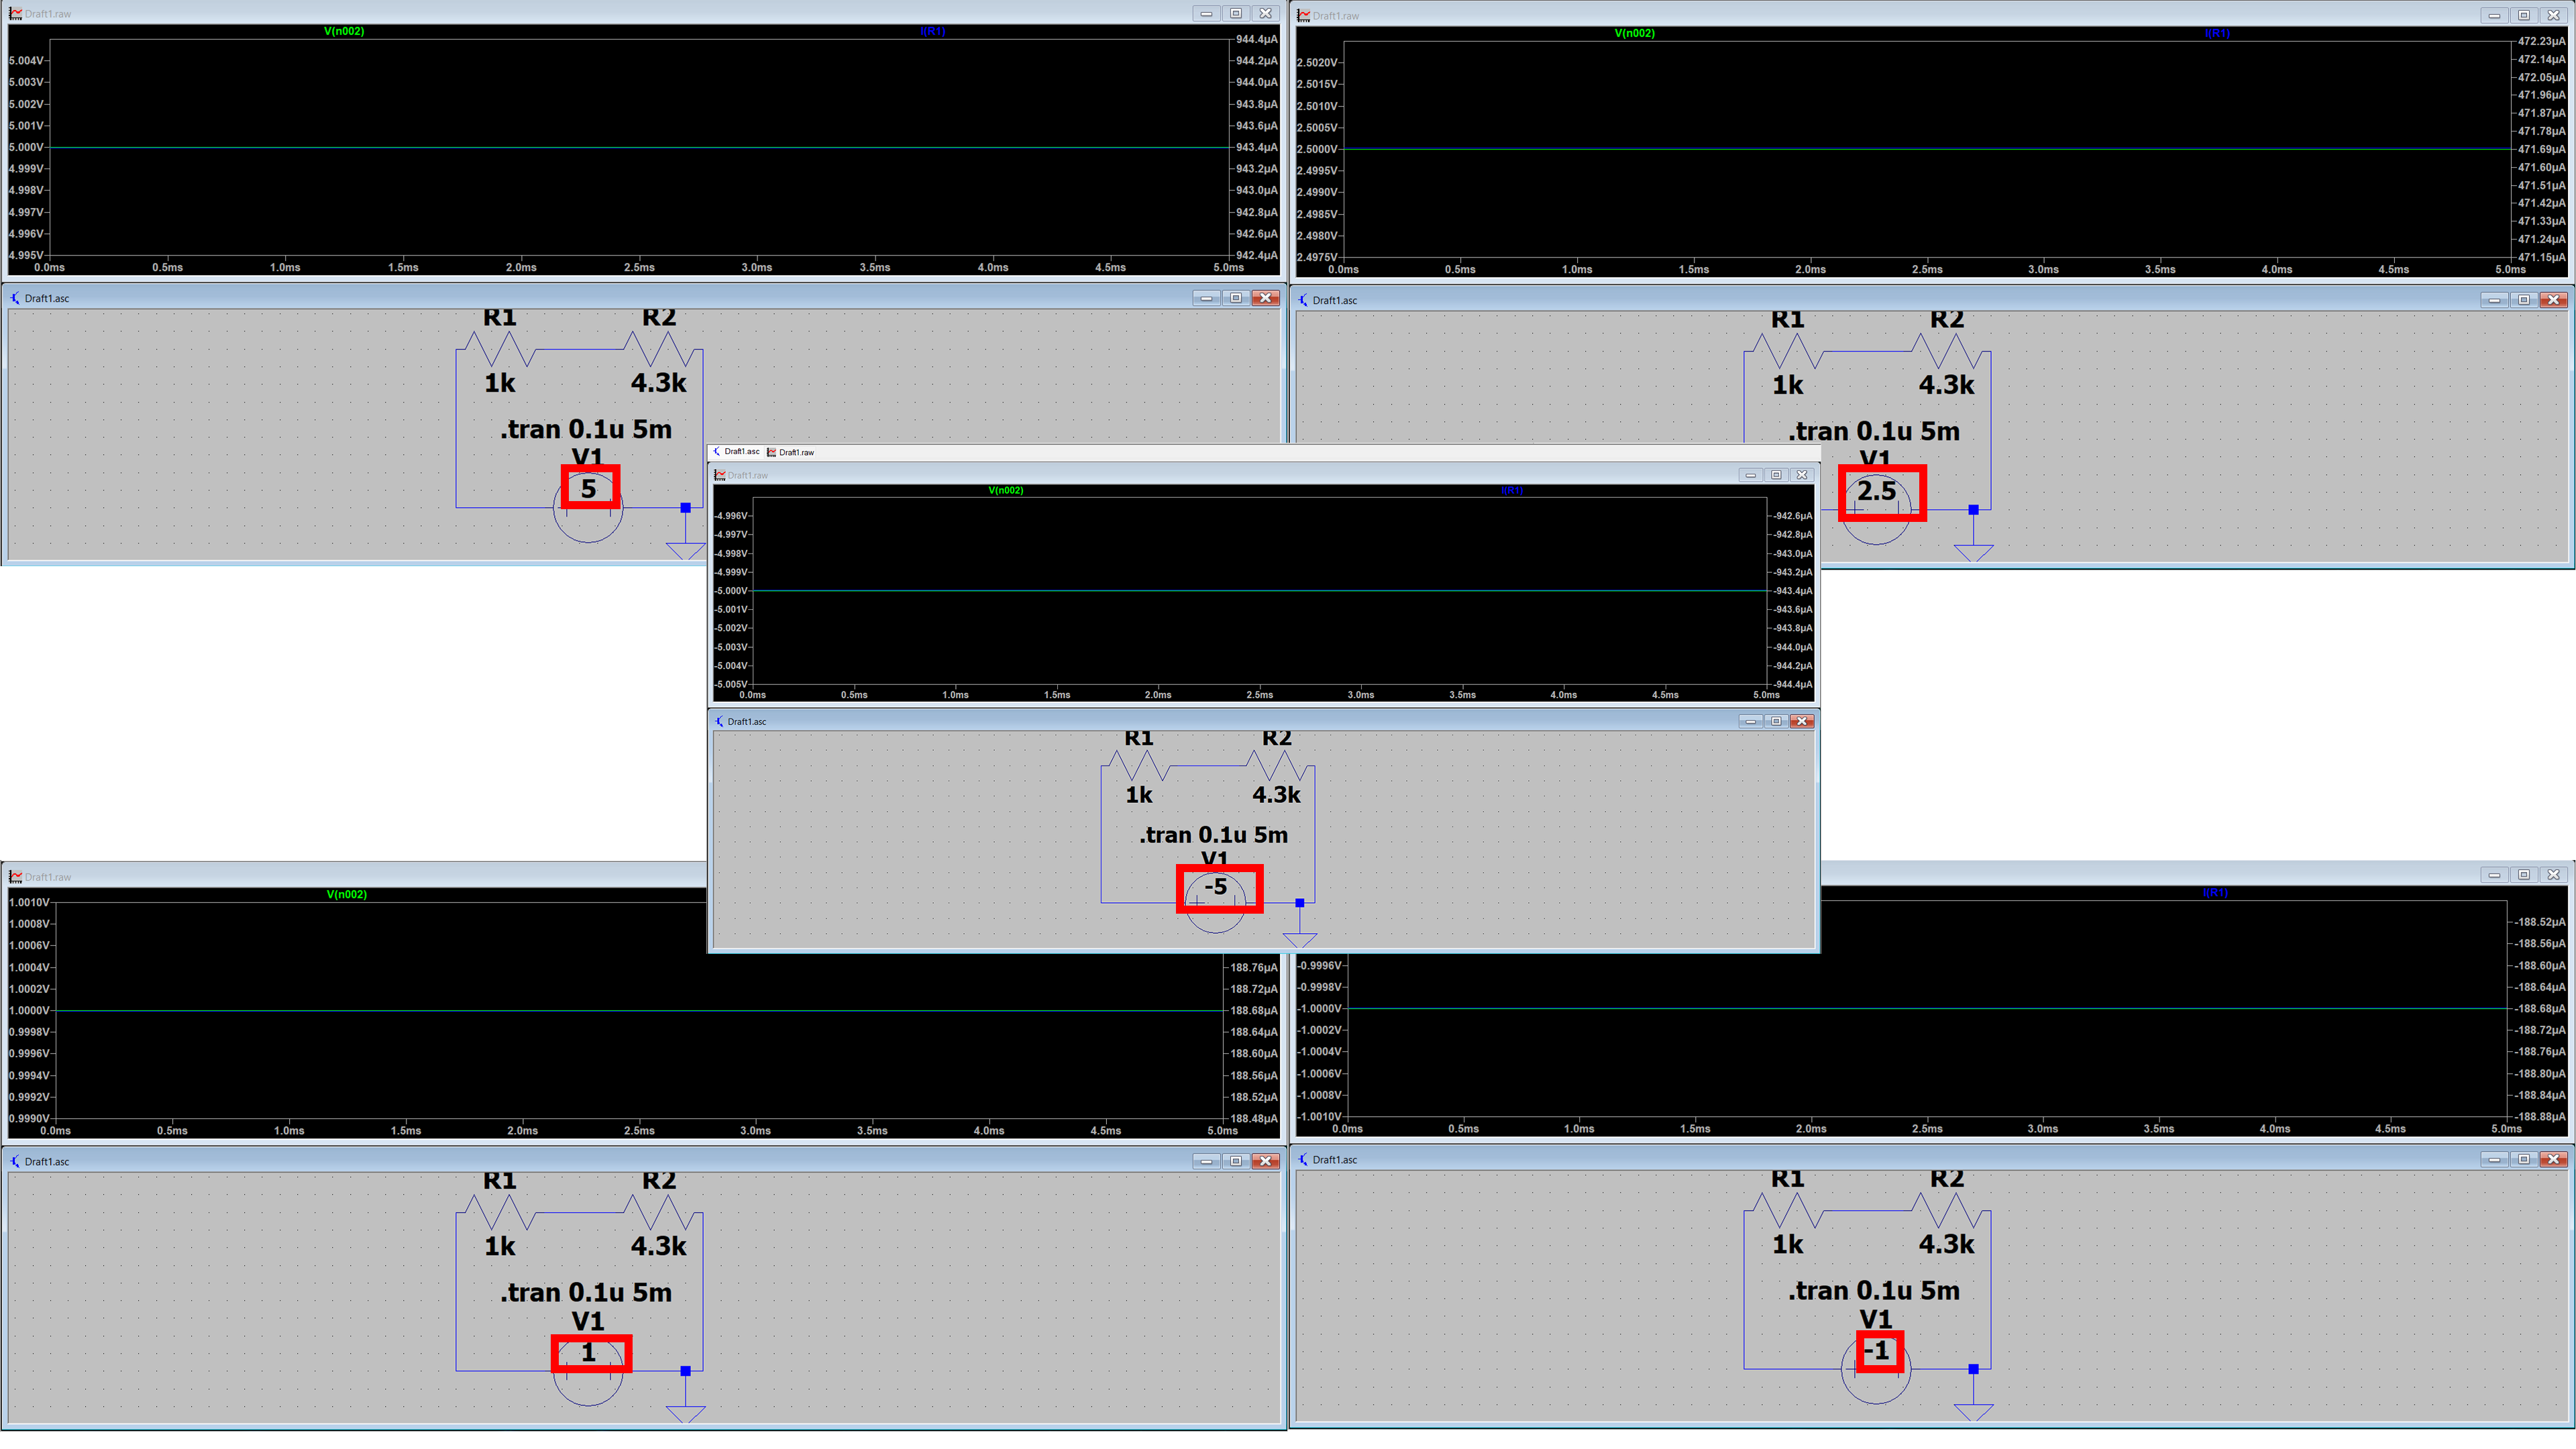
\includegraphics[width=1\textwidth]{assets/taks_2.png}
    \caption{Task\#2 Circuit Diagram \& Calculations}
\end{figure}

We choose the following values for the voltage source:
\begin{itemize}
    \item \(V_1 = -5V\)
    \item \(V_2 = -1V\)
    \item \(V_3 = 1V\)
    \item \(V_4 = 2.5V\)
    \item \(V_5 = 5V\)
\end{itemize}

\begin{center}
    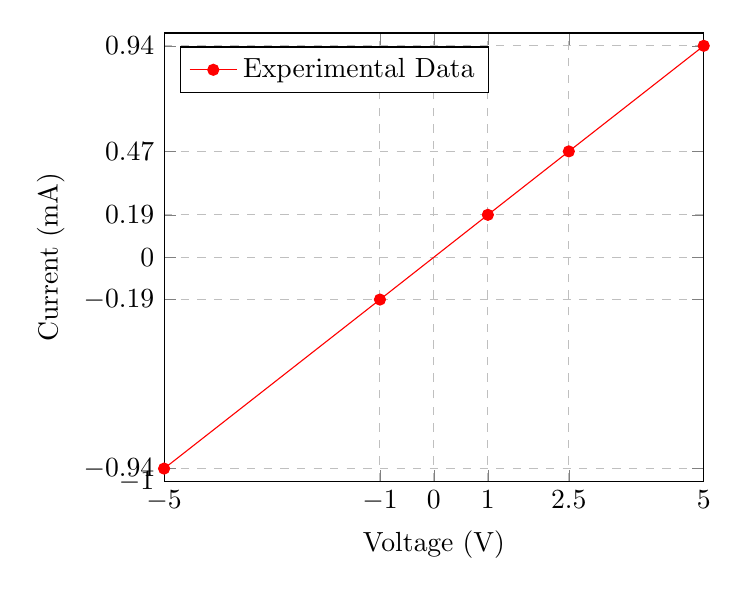
\begin{tikzpicture}
        \begin{axis}[
            xlabel={Voltage (V)},
            ylabel={Current (mA)},
            xmin=-5, xmax=5,
            ymin=-1, ymax=1,
            xtick={-5,-1,0,1,2.5,5},
            ytick={-1, -0.943, -0.189,0, 0.189, 0.472, 0.943},
            legend pos=north west,
            ymajorgrids=true,
            xmajorgrids=true,
            grid style=dashed,
        ]
            \addplot[
                color=red,
                mark=*,
            ]
            coordinates {
                (-5, -0.943)
                (-1, -0.189)
                (1, 0.189)
                (2.5, 0.472)
                (5, 0.943)
            };
            \legend{Experimental Data}
        \end{axis}
    \end{tikzpicture}
\end{center}

\newpage
\thispagestyle{plain}

\section{Exercise \#3}
\begin{figure}[h]
    \centering
    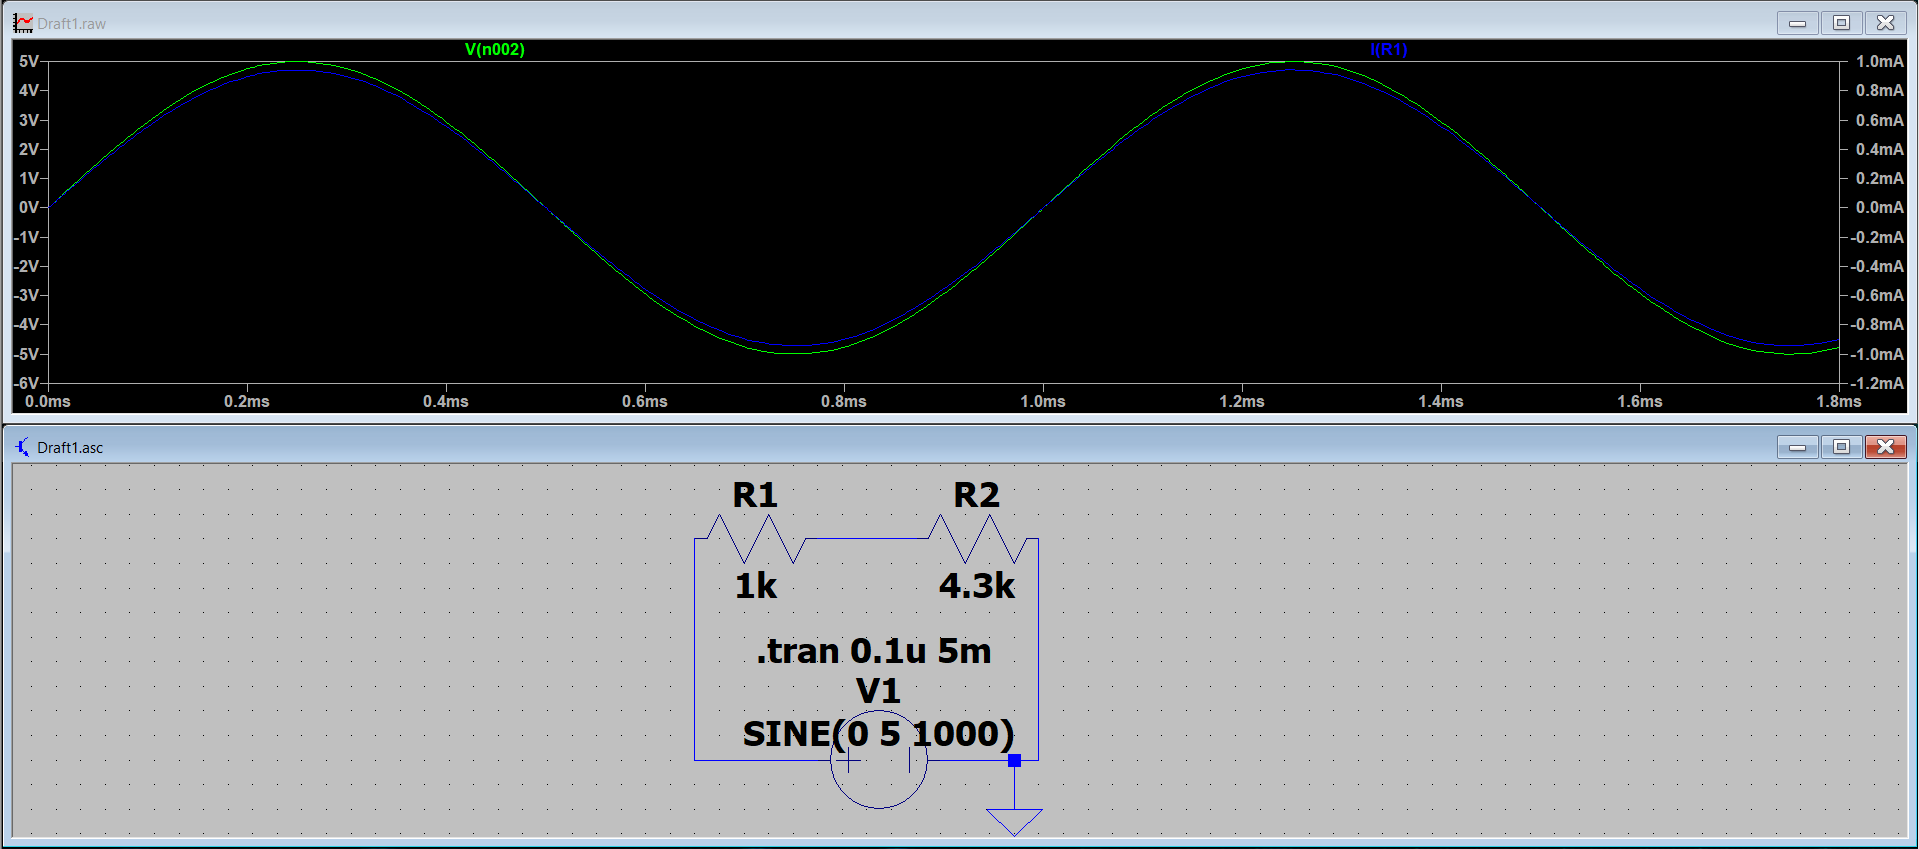
\includegraphics[width=1\textwidth]{assets/taks_3.png}
    \caption{Task\#3 Circuit Diagram \& Calculations}
\end{figure}

\newpage
\thispagestyle{plain}

\section{Exercise \#4}
\begin{figure}[h]
    \centering
    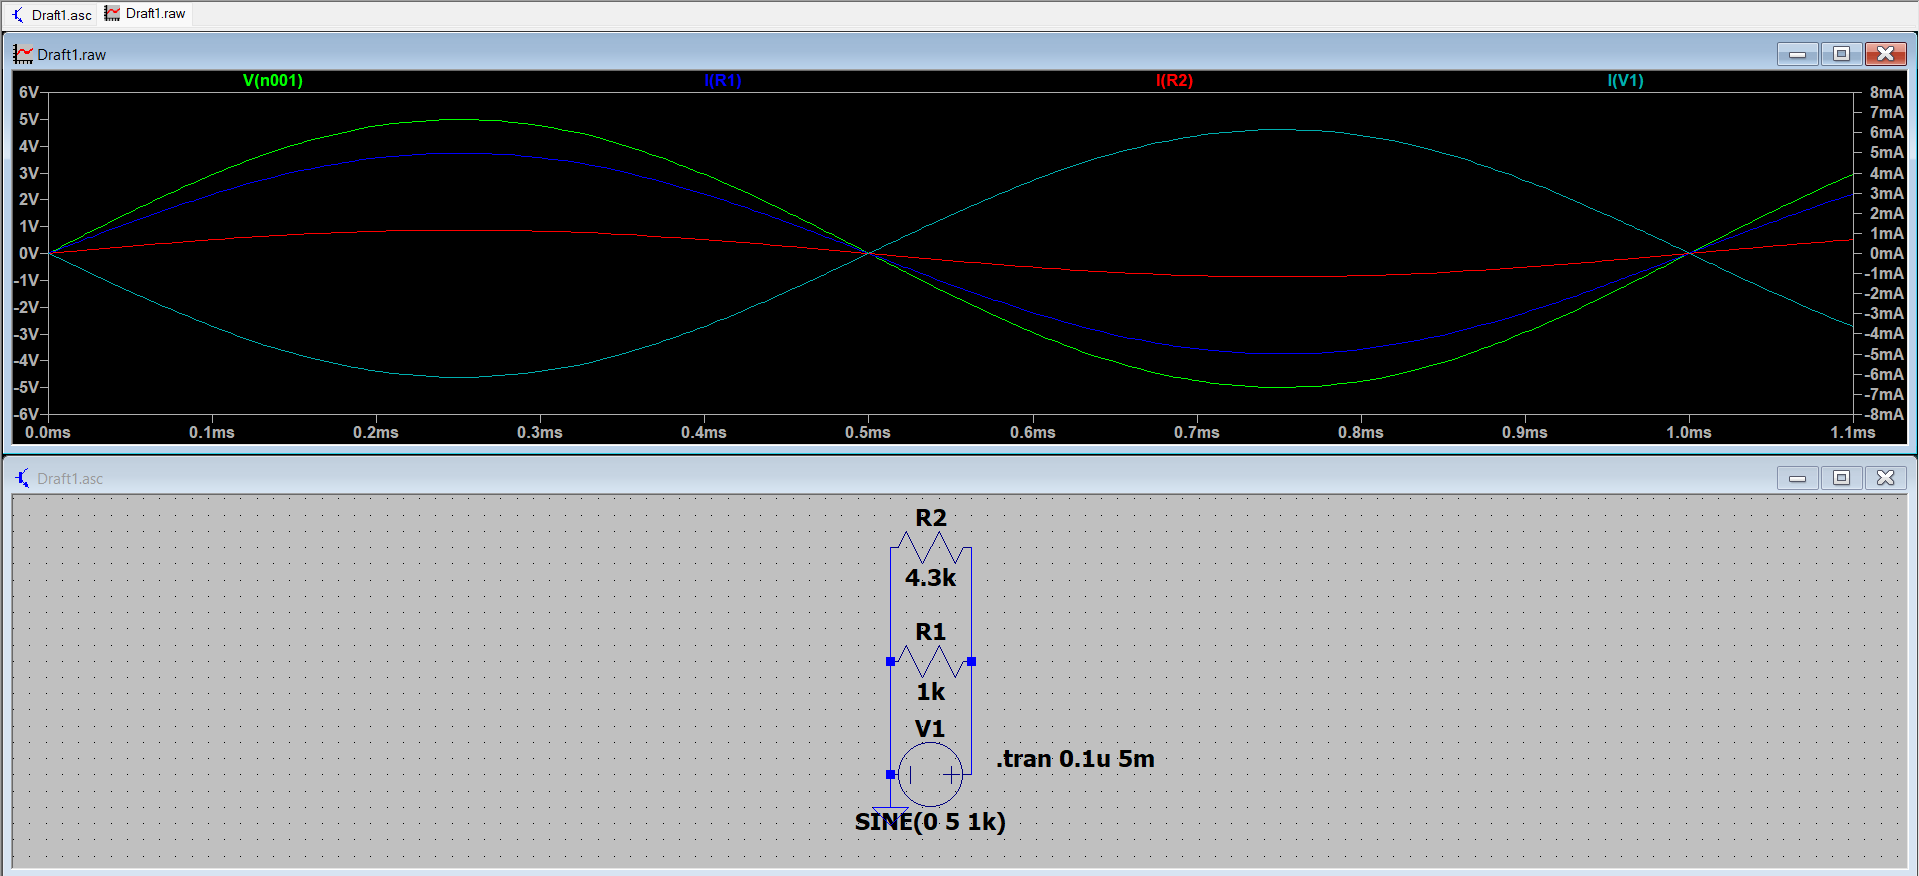
\includegraphics[width=.75\textwidth]{assets/taks_4.png}
    \caption{Task\#4 Circuit Diagram \& Calculations}
\end{figure}

First we have to calculate the equivalent resistance of the circuit. We can use the following formula to calculate the equivalent resistance of the circuit:
\begin{align*}
    R_{eq} &= \frac{R_1\times R_2}{R_1 + R_2} = \frac{1k\Omega \times 4.3k\Omega}{1k\Omega + 4.3k\Omega} \\
    &= \frac{4.3M\Omega}{5.3k\Omega} = 0.811k\Omega
\end{align*}

We choose the following values for the voltage source:
\begin{itemize}
    \item \(V_1 = -5V\)
    \item \(V_2 = -1V\)
    \item \(V_3 = 1V\)
    \item \(V_4 = 2.5V\)
    \item \(V_5 = 5V\)
\end{itemize}


\begin{center}
    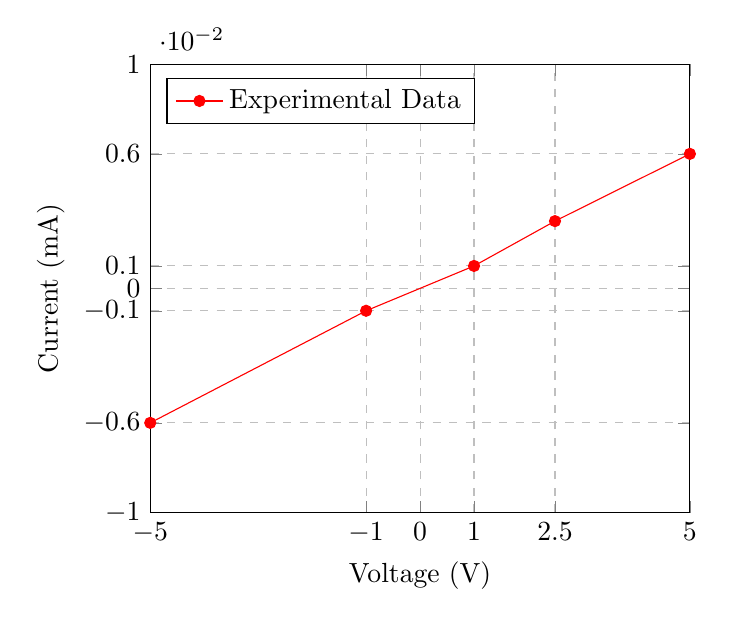
\begin{tikzpicture}
        \begin{axis}[
            xlabel={Voltage (V)},
            ylabel={Current (mA)},
            xmin=-5, xmax=5,
            ymin=-0.01, ymax=0.01,
            xtick={-5,-1,0,1,2.5,5},
            ytick={-0.01, -0.006, -0.001, 0, 0.001, 0.006, 0.01},
            legend pos=north west,
            ymajorgrids=true,
            xmajorgrids=true,
            grid style=dashed,
        ]
            \addplot[
                color=red,
                mark=*,
            ]
            coordinates {
                (-5, -0.006)
                (-1, -0.001)
                (1, 0.001)
                (2.5, 0.003)
                (5, 0.006)
            };
            \legend{Experimental Data}
        \end{axis}
    \end{tikzpicture}
\end{center}
